\subsection
{\href{http://cst.mi.fu-berlin.de/intern/19606-P-MPP/Aufgaben/040901.html}
{Aufgabe 25: Funktionsgenerator}}

Ein Programm soll eine volle Sinuskurve über den DA-Wandler auf einem
Oszilloskop zeichnen. Der Wandler wird Timer-gestützt mit Werten gefüllt.

\subsubsection*{Vorgehensweise}
Zur Lösung der Aufgabe müssen Timer und DA-Wandler initialisiert, das
Feld mit den Sinuswerten vorberechnet und eine Timer-Interrupt-Routine
zum hochzählen des Indexes definiert werden. Das Hauptprogramm ist
nach der Initialisierungsphase fertig und blockiert danach einfach in
einer Endlosschleife.

Wir arbeiten mit dem DA-Wandler 0 -- der erste der zwei vorhandenen. DAC0 wird
mit {\tt DAC12\_\-0CTL} kontrolliert und die Spannung, der analogen
Entsprechung  des Wertes in Datenregisters {\tt DAC12\_\-0DAT} liegt an
Portleitung 6.6, die selektiert wird. Der DAC wird auf eine
Referenzspannung von 3 V mit 12-Bit Auflösung programmiert. Wichtig
sind auch die Bits des ``amplifier Setting's'': der Wert 0 würde den
DAC ausschalten, also wählen wir hier Setting 7 (hohe
Wandlungsgeschwindigkeit/hoher Stromverbrauch).

Die Berechnung der Sinuswerte erfolgt mit der sin-Funktion aus math.h
(Wichtig: Vergisst man diesen Header einzubinden kompiliert das
Programm zwar, berechnet aber falsche Werte!). Alle Werte müssen auf
die 12-Bit Auflösung des DAC skaliert werden. Zum Beispiel entspricht
der Gleichspannungsoffset von 1,5V, um den die Sinuskurve auf der
Y-Achse verschoben sein soll, dem Wert $2047 = \frac{(2^{12}-1) * 1,5V} {3V}$.

Wie die Initialisierung des Timers erfolgt, wurde bereits in vorigen
Aufgaben erarbeitet. Die Timer-Interrupt-Service-Routine soll den nächsten
Sinuswert aus der vorberechneten Feld an den DAC übergeben: {\tt
  sinus[index]} auf das Datenregister {\tt
  DAC12\_\-0DAT}). Anschließend wird für das nächste Zeitinverall der
Index inkrementiert. Beim letzten Sample 100 wird wieder auf 0
gesprungen, so dass die nächste Periode ausgegeben werden kann.

\begin{center}
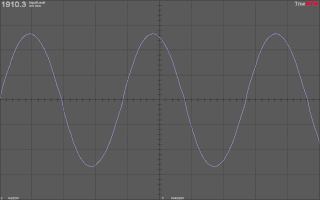
\includegraphics[scale=0.75]{aufgaben/25.png}
\end {center}

\subsubsection*{Quelltext}

\lstinputlisting[linerange=8-999,firstnumber=8,caption=aufgabe25.c]
{../MPP_WS1011/aufgaben/aufgabe25.c}

%%% Local Variables: 
%%% mode: latex
%%% TeX-master: "../Main"
%%% End: 
